\documentclass[10pt,a4paper]{article}
\usepackage{amsmath,amssymb,amsthm,graphicx}
\usepackage{amsmath,amssymb,mathtools}
\usepackage{hyperref}
\usepackage{graphicx}
\usepackage{fontspec}
\setmainfont{DejaVu Serif}
\sloppy
\setlength{\emergencystretch}{3em}
\title{Non-simple Venn arrangement graphs with no perfect matching}
\author{Sofia Brenner, Linda Kleist, Torsten Mütze, Christian Rieck, Francesco Verciani}
\date{doi:10.4230/LIPIcs.SoCG.2026.22; CC BY 4.0}
\begin{document}
\maketitle
\noindent\textit{Editorial scope.} An inductive cylindrical wire-diagram construction controls every crossing and curve order; splitting two full crossings creates an oversized independent set in an even-order arrangement graph, giving the authors analytic obstruction for all n>=4. Original published author counterexample only. Complete constructive proof is in official CCBY material; no software enumeration used for this counted claim.\par\medskip
\noindent\textit{Allowed standard prerequisites (editorial).}\begin{itemize}
\item Venn diagram duality, Hall and Tutte perfect-matching obstructions. Original definitions and citations preserved. Source-specific ladders, gluing, explicit base witness and inductive wire-diagram construction fully retained.
\end{itemize}\medskip
% BEGIN S1
\par\medskip\noindent\textbf{1 Introduction}\par
% BEGIN S1.p1
Venn diagrams are a popular tool to illustrate the relations between sets and operations on them, such as union and intersection, or the well-known inclusion-exclusion principle. Historically, these diagrams were introduced by John Venn [18] (1834–1923) in the context of formal logic. Most illustrations that one finds depict the Venn diagram with three sets represented by unit circles; see Figure 1 (a). It may even come as a surprise that Venn diagrams exist for any number of sets, not just three. Formally, an $n$-Venn diagram is a collection of $n$ simple closed curves in the plane that intersect in only finitely many points and create exactly $2^{n}$ regions, one for every possible combination of being inside or outside of each of the $n$ curves. Figures 1 (b)+(c) display diagrams with $n=4$ and $n=5$ curves, respectively.
\par
\par
% END S1.p1
% BEGIN S1.p2
A Venn diagram is simple if at most two of the $n$ curves intersect in any point: The three diagrams in the top row of Figure 1 are simple, whereas the three diagrams in the bottom row are non-simple. An easy application of Euler’s formula shows that a simple Venn diagram has exactly $2^{n}-2$ crossings, whereas non-simple diagrams may have much fewer. For humans, simple Venn diagrams tend to be easier to read than non-simple diagrams.
\par
\par
% END S1.p2
% BEGIN S1.F1
\begin{center}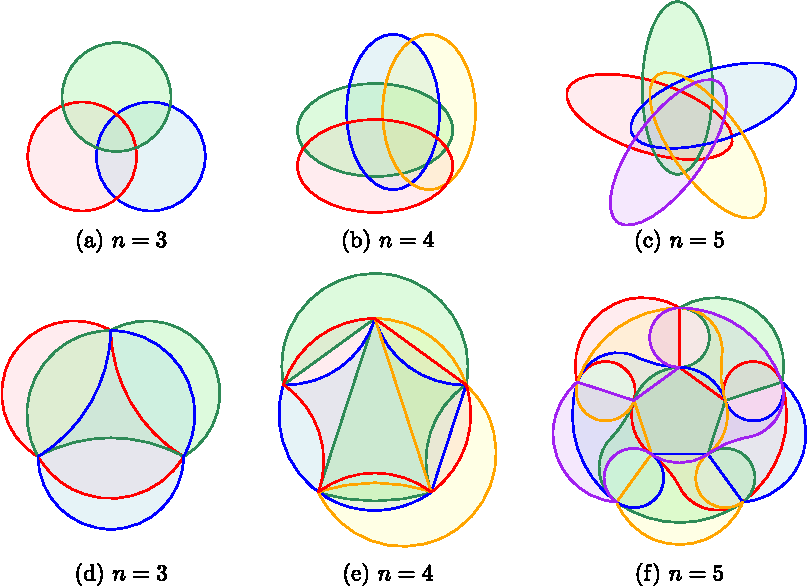
\includegraphics[width=0.7\linewidth,height=0.38\textheight,keepaspectratio]{graphics-page-1.pdf2svg.pdf}\end{center}
\par
 Figure 1: Venn diagrams with $n=3,4,5$ curves: (a), (b), (c) are simple, whereas (d), (e), (f) are non-simple; (a), (b), (d) are reducible, whereas (c), (e), (f) are irreducible; (a), (b), (c), (d) are monotone, whereas (e), (f) are not monotone; (a), (b), (c), (d), (f) are exposed, whereas (e) is not exposed. 
% END S1.F1
% BEGIN S1.SS1
\par\medskip\noindent\textbf{1.1 Winkler’s conjecture}\par
% BEGIN S1.SS1.p1
In 1984, Peter Winkler [20] raised the following intriguing conjecture about extending a simple Venn diagram by adding one curve to it.
\par
\par
% END S1.SS1.p1
% BEGIN Thmtheorem1
\par\medskip\noindent\textbf{Conjecture 1.}\par
Every simple $n$-Venn diagram can be extended to a simple $(n+1)$-Venn diagram by the addition of a suitable curve.
\par
\par
\par
% END Thmtheorem1
% BEGIN S1.SS1.p2
He also mentioned the conjecture as an unsolved open problem in his popular book [21] on mathematical puzzles, and reiterated it in his “Puzzled” column [22] in the Communications of the ACM. The conjecture is also listed as the first open problem in Ruskey and Weston’s inspiring survey [15] on Venn diagrams.
\par
\par
% END S1.SS1.p2
% BEGIN S1.SS1.p3
For small cases, the conjecture is easily verifiable by hand for all simple Venn diagrams on $n\in\{3,4,5\}$ curves, simply because there are so few of them; the 20 diagrams for $n=5$ can be found in [6, 10]. Another class of Venn diagrams for which the conjecture is easily seen to be true are reducible diagrams. An $n$-Venn diagram is reducible if one of its curves can be removed so that the remaining $n-1$ curves form an $(n-1)$-Venn diagram. Otherwise the diagram is called irreducible. The diagram in Figure 1 (c) is irreducible. If a diagram is reducible, then the curve $C$ that can be removed splits every region of the resulting $(n-1)$-Venn diagram into two, and therefore this curve touches every region in the $n$-Venn diagram. We can thus add an $(n+1)$st curve by following the curve $C$ and subdividing every region into two, changing sides along $C$ exactly once along every segment between two consecutive crossings. Thus, the interesting instances of Conjecture 1 are irreducible diagrams.
\par
\par
% END S1.SS1.p3
% BEGIN S1.SS1.p4
Grünbaum [9] modified Winkler’s conjecture, dropping the requirement for the diagrams to be simple. This makes the problem harder in the sense that more diagrams are allowed, but easier in the sense that there is substantially more freedom when adding the new curve. This variant of the conjecture was proved subsequently by Chilakamarri, Hamburger and Pippert [4], by using a straightforward reduction to a classical result of Whitney [19].
\par
\par
% END S1.SS1.p4
% BEGIN S1.SS1.SSS1
\par\medskip\noindent\textbf{1.1.1 Translation to a Hamilton cycle problem}\par
% BEGIN S1.SS1.SSS1.p1
Problems on Venn diagrams such as Winkler’s conjecture are best discussed by considering the dual graph of the Venn diagram, i.e., the plane graph that has a vertex inside every region, and edges connecting vertices corresponding to neighboring regions; see Figure 2. For this, we consider the $n$-dimensional hypercube $Q_{n}$, or $n$-cube for short, the graph formed by all bitstrings of length $n$, with an edge between any two bitstrings that differ in a single bit. The dual graph $Q(D)$ of a simple $n$-Venn diagram $D$ satisfies the following properties:
\par
  1  
It is a connected subgraph of $Q_{n}$ that is also spanning, i.e., all $2^{n}$ vertices are present. Specifically, the vertex in $Q(D)$ corresponding to a region of the diagram $D$ is the characteristic vector of the inside/outside relation with respect to each curve, where 0 and 1 represent outside and inside, respectively.111When considering the diagram in the plane, then the inside and outside of a curve $C$ are the bounded and unbounded region of $\mathbb{R}^{2}\setminus C$, respectively.
\par
\par
  2  
It is a plane quadrangulation, i.e., it is drawn in the plane without edge crossings, and every face (including the outer face) is a 4-cycle.
\par
\par
  3  
For every position $i\in\{1,\ldots,n\}$ and every bit $b\in\{0,1\}$, the subgraph of $Q(D)$ induced by all vertices $x$ with $x_{i}=b$ is connected.
\par
\par
Conversely, the dual of any subgraph of $Q_{n}$ satisfying these properties is an $n$-Venn diagram.
\par
\par
% END S1.SS1.SSS1.p1
% BEGIN S1.F2
\begin{center}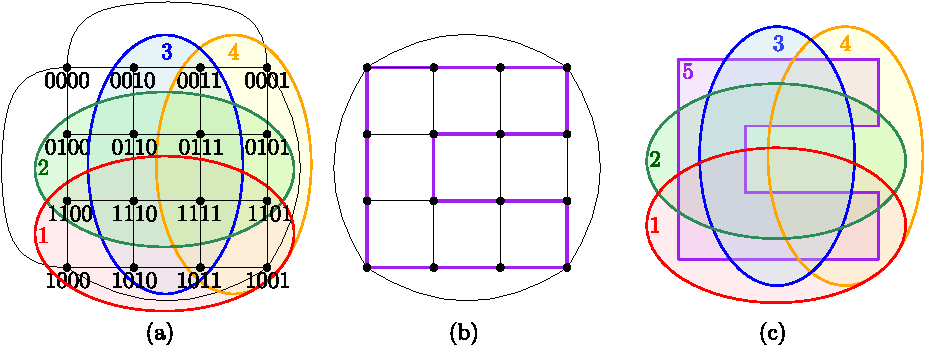
\includegraphics[width=0.7\linewidth,height=0.38\textheight,keepaspectratio]{graphics-page-14.pdf2svg.pdf}\end{center}
\par
 Figure 2: (a) A 4-Venn diagram and its dual graph, a 4-Venn quadrangulation; (b) a Hamilton cycle in the quadrangulation; (c) the 5-Venn diagram obtained from (a) by adding the curve corresponding to the Hamilton cycle in (b). 
% END S1.F2
% BEGIN S1.SS1.SSS1.p2
We refer to subgraphs of $Q_{n}$ satisfying 1–3, which are the duals of $n$-Venn diagrams, as $n$-Venn quadrangulations.
\par
\par
% END S1.SS1.SSS1.p2
% BEGIN S1.SS1.SSS1.p3
Extending the diagram $D$ by a single curve means that the new curve has to enter and leave every region of $D$ exactly once, splitting it into two, one of them inside and the other one outside the newly added curve. This corresponds to traversing a Hamilton cycle in the dual graph $Q(D)$, i.e., a cycle in the graph that visits every vertex exactly once; see Figure 2 (b)+(c).
\par
\par
% END S1.SS1.SSS1.p3
% BEGIN S1.SS1.SSS1.p4
Conjecture 1 can thus be restated equivalently as follows: For $n\geq 2$, every $n$-Venn quadrangulation admits a Hamilton cycle.
\par
\par
% END S1.SS1.SSS1.p4
% END S1.SS1.SSS1
% BEGIN S1.SS1.SSS2
\par\medskip\noindent\textbf{1.1.2 The counterexamples}\par
% BEGIN S1.SS1.SSS2.p1
As $Q_{n}$ is a bipartite graph, Venn quadrangulations are bipartite, too. A necessary condition for the existence of a Hamilton cycle in a bipartite graph is the existence of a perfect matching. We provide counterexamples to Conjecture 1 by constructing, for every $n\geq 6$, an $n$-Venn quadrangulation that has no perfect matching and thus no Hamilton cycle. One of our counterexamples for $n=6$ is shown in Figure 3.
\par
\par
% END S1.SS1.SSS2.p1
% BEGIN S1.F3
\begin{center}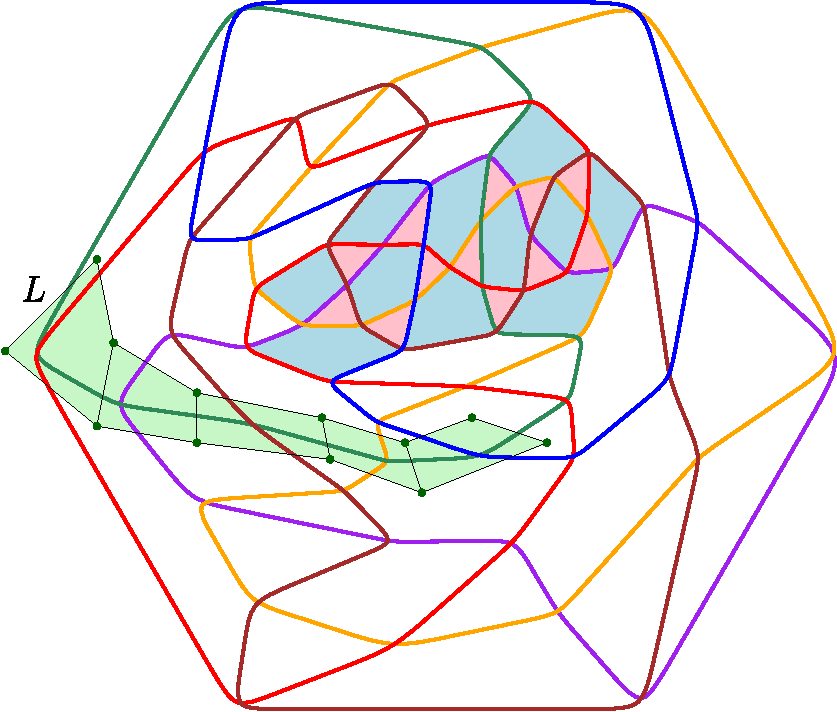
\includegraphics[width=0.7\linewidth,height=0.38\textheight,keepaspectratio]{counter6.pdf2svg.pdf}\end{center}
\begin{center}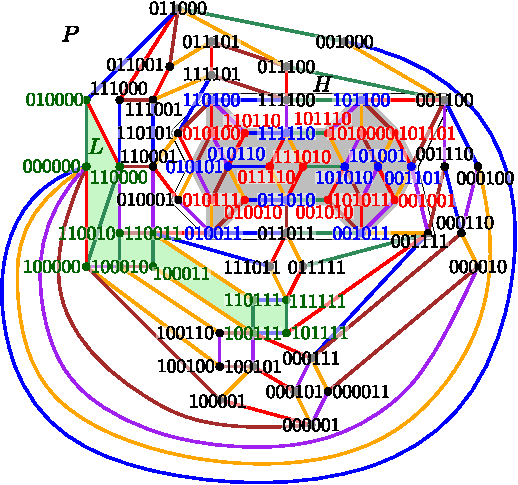
\includegraphics[width=0.7\linewidth,height=0.38\textheight,keepaspectratio]{counter6-dual.pdf2svg.pdf}\end{center}
  Figure 3: (Left) A counterexample to Winkler’s conjecture for $n=6$, namely a simple 6-Venn diagram that cannot be extended to a simple 7-Venn diagram by adding a suitable curve. Highlighted are 12 red regions that are surrounded by only 11 blue regions, which is a local obstruction for extendability.333This drawing was produced using a SageMath program [16] developed by Manfred Scheucher for his and Felsner’s work [7] on pseudocircle arrangements. We used this program with Scheucher’s permission, using as input the 6-Venn quadrangulation on the right. (Right) The dual graph of the diagram on the left, namely a 6-Venn quadrangulation $P$ that has no perfect matching and hence no Hamilton cycle. Edges are colored according to the colors of the curves. The highlighted subgraph $H$ contains a subset of 12 red vertices in one partition class and their 11 blue neighbors, witnessing the non-existence of a perfect matching. The green subgraph $L$ is the ladder used for extending the counterexample to all values of $n>6$, and all those extensions contain a copy of $H$. 
% END S1.F3
% BEGIN Thmtheorem2
\par\medskip\noindent\textbf{Theorem 2.}\par
For every $n\geq 6$ there is an $n$-Venn quadrangulation that has no perfect matching and hence no Hamilton cycle. Its dual is a simple $n$-Venn diagram that cannot be extended to a simple $(n+1)$-Venn diagram by adding a suitable curve.
\par
\par
\par
% END Thmtheorem2
% BEGIN S1.SS1.SSS2.p2
As mentioned before, for $n\leq 5$ all simple $n$-Venn diagrams are extendable, so Theorem 2 is best possible in the sense that the counterexamples for $n=6$ are minimal. In fact, as part of our proof of Theorem 2 we computed all distinct 6-Venn diagrams and analyzed their properties, summarized in the next theorem, Figure 4 and Table 1. Specifically, we consider two diagrams the same if they differ only by mirroring and/or stereographic projection. Equivalently, we count their dual $n$-Venn quadrangulations up to graph isomorphism. Prior to this work, the number of simple $n$-Venn diagrams was only known up to $n\leq 5$. Specifically, for each $n\leq 4$ there is only one, and for $n=5$ there are 20 [6, 10].
\par
\par
% END S1.SS1.SSS2.p2
% BEGIN S1.SS1.SSS2.p3
To state the next theorem, we define a few relevant properties. A $k$-region in an $n$-Venn diagram is a region that lies inside of exactly $k$ of the $n$ curves (and outside of the remaining $n-k$ curves). A monotone Venn diagram is one in which for every $0<k<n$, every $k$-region is adjacent to both a $(k-1)$-region and a $(k+1)$-region. Bultena, Grünbaum and Ruskey [3] proved that monotone diagrams are precisely the ones that can be drawn such that every curve has a convex shape. An exposed diagram is one in which the outer region is bounded by all $n$ curves. It is not hard to see that any monotone diagram is also exposed. Chilakamarri, Hamburger and Pippert [5] constructed $n$-Venn diagrams for every $n$ in which all regions are (combinatorial) triangles, quadrangles or pentagons, in particular, they are not exposed for $n\geq 6$.
\par
\par
% END S1.SS1.SSS2.p3
% BEGIN S1.F4
\begin{center}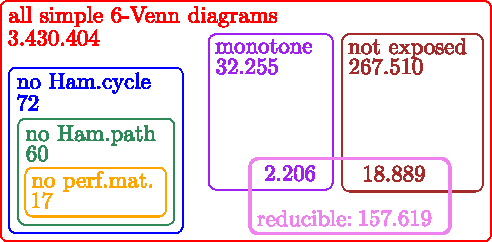
\includegraphics[width=0.7\linewidth,height=0.38\textheight,keepaspectratio]{graphics-page-10.pdf2svg.pdf}\end{center}
\par
 Figure 4: Census of 6-Venn diagrams and their properties stated in Theorem 3, visualized as an Euler diagram. The sizes of the boxes are not to scale. 
% END S1.F4
% BEGIN S1.SS1.SSS2.p4
As a consequence of Theorem 3, there are 6-Venn quadrangulations (in total $72-17=55$ many) that have a perfect matching but no Hamilton cycle, and 6-Venn quadrangulations (in total $60-17=43$ many) that have a perfect matching but no Hamilton path.
\par
\par
% END S1.SS1.SSS2.p4
% BEGIN S1.SS1.SSS2.p5
The programs we used for computing all simple 6-Venn diagrams and the result files with all 6-Venn quadrangulations are available for download [2].
\par
\par
% END S1.SS1.SSS2.p5
% END S1.SS1.SSS2
% END S1.SS1
% BEGIN S1.SS2
\par\medskip\noindent\textbf{1.2 Pruesse and Ruskey’s conjecture}\par
% BEGIN S1.SS2.p1
While working on Winkler’s conjecture, Pruesse and Ruskey [14] considered the question of finding a Hamilton cycle not in the dual graph of a Venn diagram, but in the arrangement graph whose vertices are the crossings of the curves, and curve segments between consecutive crossings form the edges; see Figure 5. Note that these graphs may have multiple edges.
\par
\par
% END S1.SS2.p1
% BEGIN S1.F5
\begin{center}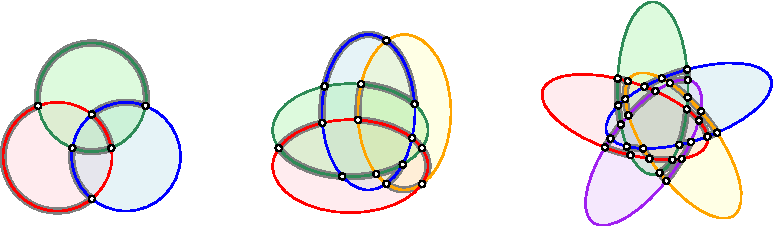
\includegraphics[width=0.7\linewidth,height=0.38\textheight,keepaspectratio]{graphics-page-2.pdf2svg.pdf}\end{center}
\par
 Figure 5: Hamilton cycles in the arrangement graphs of the Venn diagrams from Figure 1 (a)–(c). 
% END S1.F5
% BEGIN Thmtheorem4
\par\medskip\noindent\textbf{Theorem 4 ([14, Cor. 1]).}\par
For $n\geq 2$, the arrangement graph of any simple $n$-Venn diagram has a Hamilton cycle.
\par
\par
\par
% END Thmtheorem4
% BEGIN S1.SS2.p2
Their proof demonstrates that the arrangement graph of a simple Venn diagram is 4-connected for $n\geq 3$, and thus a well-known theorem of Tutte [17] implies Hamiltonicity. Pruesse and Ruskey also conjectured that their result generalizes to non-simple diagrams.
\par
\par
% END S1.SS2.p2
% BEGIN Thmtheorem5
\par\medskip\noindent\textbf{Conjecture 5 ([14, Conj. 1]).}\par
For $n\geq 2$, the arrangement graph of any (not necessarily simple) $n$-Venn diagram has a Hamilton cycle.
\par
\par
\par
% END Thmtheorem5
% BEGIN S1.SS2.SSS1
\par\medskip\noindent\textbf{1.2.1 The counterexamples}\par
% BEGIN S1.SS2.SSS1.p1
We disprove Conjecture 5 by providing counterexamples for all $n\geq 4$. Similarly to Theorem 2, our counterexamples have an even number of vertices and do not admit a perfect matching, which would be necessary for having a Hamilton cycle. One of the counterexamples for $n=4$ is shown in Figure 6.
\par
\par
% END S1.SS2.SSS1.p1

% BEGIN Thmtheorem6
\par\medskip\noindent\textbf{Theorem 6.}\par
For every $n\geq 4$, there is a non-simple $n$-Venn diagram whose arrangement graph has an even number of vertices and no perfect matching, and hence no Hamilton cycle.
\par
\par
\par
% END Thmtheorem6

% BEGIN S1.F6
\begin{center}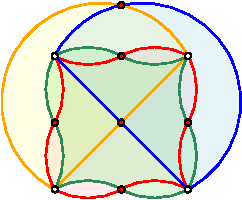
\includegraphics[width=0.7\linewidth,height=0.38\textheight,keepaspectratio]{graphics-page-3.pdf2svg.pdf}\end{center}
\par
 Figure 6: A counterexample to Pruesse and Ruskey’s conjecture for $n=4$, namely a non-simple 4-Venn diagram whose arrangement graph has an even number of vertices and no perfect matching, and hence no Hamilton cycle. The 6 red vertices form an independent set, and the complement has only 4 vertices, witnessing the non-existence of a perfect matching. 
% END S1.F6
% BEGIN S1.SS2.SSS1.p2
We remark that the counterexamples constructed in the proof of Theorem 6, including the one shown in Figure 6, are actually monotone. With straightforward modifications the diagrams can also be made crossing, i.e., such that whenever two curves meet, they cross.
\par
\par
% END S1.SS2.SSS1.p2
% END S1.SS2.SSS1
% END S1.SS2
% END S1
% BEGIN S2
\par\medskip\noindent\textbf{2 Proof of Theorem 2}\par
% BEGIN S2.p1
Our first lemma describes a technique to construct a simple $(n+1)$-Venn diagram from a simple $n$-Venn diagram, by carefully gluing together two slitted copies of the smaller diagram, surrounding one of the copies with an additional curve. In this process, a certain local substructure $H$ is preserved, and we will later apply the lemma by taking for $H$ a substructure that witnesses non-extendability. The lemma is conveniently stated in the language of the dual Venn quadrangulations.
\par
\par
% END S2.p1
% BEGIN S2.p2
If $e$ is an edge of $Q_{n}$ whose end vertices differ in the $k$th bit, then we refer to $k$ as the type of the edge $e$. A ladder in an $n$-Venn quadrangulation is a subgraph $L$ on pairwise distinct vertices $x_{1},\ldots,x_{n}$ and $y_{1},\ldots,y_{n}$ such that $x_{1}=0^{n}$, $y_{n}=1^{n}$, for some $k\in[n]:=\{1,\ldots,n\}$ all pairs $(x_{i},y_{i})$ for $i=1,\ldots,n$ are edges of type $k$ in $L$, and for $i=1,\ldots,n-1$ all pairs $(x_{i},x_{i+1})$ and $(y_{i},y_{i+1})$ are edges of arbitrary type in $L$; see Figure 7. A ladder for $n=6$ is highlighted in green in Figure 3. We note that in a Venn quadrangulation, every 4-cycle also bounds a face, i.e., either the inside or outside of the 4-cycle is empty, because otherwise condition 3 would be violated. Consequently, in a ladder, each of the 4-cycles $(x_{i},x_{i+1},y_{i+1},y_{i})$ for $i=1,\ldots,n-1$ bounds a 4-face.
\par
\par
% END S2.p2
% BEGIN S2.F7
\begin{center}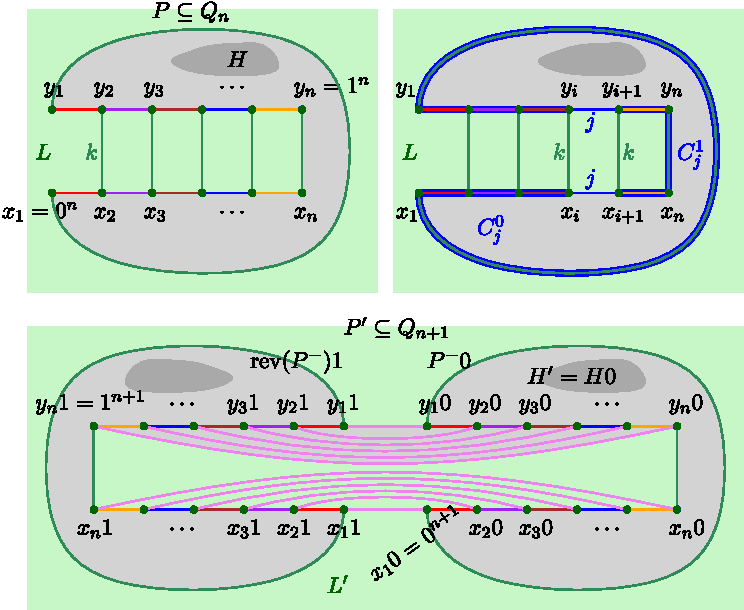
\includegraphics[width=0.7\linewidth,height=0.38\textheight,keepaspectratio]{graphics-page-11.pdf2svg.pdf}\end{center}
\par
 Figure 7: Illustration of Lemma 7. 
% END S2.F7
% BEGIN Thmtheorem7
\par\medskip\noindent\textbf{Lemma 7.}\par
Consider an $n$-Venn quadrangulation $P$ that contains a ladder $L$ and a subgraph $H$ with $L\cap H=\emptyset$. Then there is an $(n+1)$-Venn quadrangulation $P^{\prime}$ that contains a ladder $L^{\prime}$ and a copy $H^{\prime}$ of $H$ such that $L^{\prime}\cap H^{\prime}=\emptyset$.
\par
\par
\par
% END Thmtheorem7
% BEGIN S2.p3
The proof of Lemma 7 is illustrated in Figure 7.
\par
\par
% END S2.p3
% BEGIN S2.SS0.SSS0.P0.SPx1
\par\medskip\noindent\textbf{Proof.}\par
% BEGIN S2.SS0.SSS0.P0.SPx1.p1
Let $x_{1},\ldots,x_{n}$ and $y_{1},\ldots,y_{n}$ be the vertices of the ladder $L$ in $P$ as defined before, and let $k\in[n]$ be the type of the edges $(x_{i},y_{i})$ for $i=1,\ldots,n$. We write $C$ for the outer cycle of $L$, i.e., for the graph $C:=L\setminus\{(x_{i},y_{i})\mid i=2,\ldots,n-1\}$. Note that in every 4-cycle of a Venn quadrangulation, there are edges of exactly two different types, and opposite edges have the same type. Consequently, both edges $(x_{i},x_{i+1})$ and $(y_{i},y_{i+1})$ of $L$ (and $C$) have the same type for $i=1,\ldots,n-1$, and because of the condition $x_{1}=0^{n}$ and $y_{n}=1^{n}$, every type $j\in[n]\setminus\{k\}$ appears for exactly one pair of opposite edges $(x_{i},x_{i+1})$ and $(y_{i},y_{i+1})$ for some $i=1,\ldots,n-1$. We write $C_{j}^{0}$ and $C_{j}^{1}$ for the two connected subgraphs of $C$ obtained from $C$ by removing both edges $(x_{i},x_{i+1})$ and $(y_{i},y_{i+1})$, such that the first one contains the vertex $x_{1}=0^{n}$ and the second one contains the vertex $y_{n}=1^{n}$.
\par
\par
% END S2.SS0.SSS0.P0.SPx1.p1
% BEGIN S2.SS0.SSS0.P0.SPx1.p2
We assume w.l.o.g. that the 4-cycle $(x_{1},x_{2},y_{2},y_{1})$ bounds the outer face of $P$. Let $P^{-}$ be the graph obtained from $P$ by removing the edges $(x_{i},y_{i})$ of the ladder $L$ for all $i=2,\ldots,n-1$. Let $\operatorname{rev}(P^{-})$ denote the plane graph obtained from $P^{-}$ by mirroring. Appending a 0-bit to all vertices of $P^{-}$ and a 1-bit to all vertices of $\operatorname{rev}(P^{-})$ gives the graphs $P^{-}0$ and $\operatorname{rev}(P^{-})1$. We let $P^{\prime}$ be the plane graph obtained by connecting $P^{-}0$ and $\operatorname{rev}(P^{-})1$ via $2n$ additional type-$(n+1)$ edges $(x_{j}0,x_{j}1)$ and $(y_{j}0,y_{j}1)$ for all $j=1,\ldots,n$. It is straightforward to check that $P^{\prime}$ satisfies conditions 1–3. In particular, the connectivity condition 3 is ensured via the subgraphs $C_{j}^{0}$ and $C_{j}^{1}$ for all bit positions $j\in[n]\setminus\{k\}$, and for the bit position $k$ it is ensured via the subgraphs $C0$ and $C1$.
\par
\par
% END S2.SS0.SSS0.P0.SPx1.p2
% BEGIN S2.SS0.SSS0.P0.SPx1.p3
Note that $P^{\prime}$ contains a ladder $L^{\prime}$ on the vertices $x_{1}0,\ldots,x_{n}0,y_{n}0$ and $x_{1}1,\ldots,x_{n}1,y_{n}1$. Clearly, $H0$ is a copy of $H$ in $P^{\prime}$ that is disjoint from $L^{\prime}$. $\hfill\blacktriangleleft$
\par
\par
% END S2.SS0.SSS0.P0.SPx1.p3
% BEGIN S2.SS0.SSS0.P0.SPx1.p4
We are now ready to prove Theorem 2.
\par
\par
% END S2.SS0.SSS0.P0.SPx1.p4
% END S2.SS0.SSS0.P0.SPx1
% BEGIN S2.SS0.SSS0.P0.SPx2
\par\medskip\noindent\textbf{Proof of Theorem 2.}\par
% BEGIN S2.SS0.SSS0.P0.SPx2.p1
The 6-Venn quadrangulation $P$ from Figure 3 has no perfect matching, as witnessed by the marked subgraph $H$. Specifically, $H$ contains a subset of 12 vertices from one partition class (marked red) whose neighborhood (marked blue) has only size 11. This is the easy direction of Hall’s marriage theorem.
\par
\par
% END S2.SS0.SSS0.P0.SPx2.p1
% BEGIN S2.SS0.SSS0.P0.SPx2.p2
Repeatedly applying Lemma 7 to $P$ with the subgraph $H$ and the ladder $L$ marked in Figure 3 yields an $n$-Venn quadrangulation without perfect matching for all $n>6$. This completes the proof. $\hfill\blacktriangleleft$
\par
\par
% END S2.SS0.SSS0.P0.SPx2.p2
% END S2.SS0.SSS0.P0.SPx2
% END S2
% BEGIN S4
\par\medskip\noindent\textbf{4 Proof of Theorem 6}\par
% BEGIN S4.p1
In this section, we prove Theorem 6.
\par
\par
% END S4.p1
% BEGIN S4.F10
\begin{center}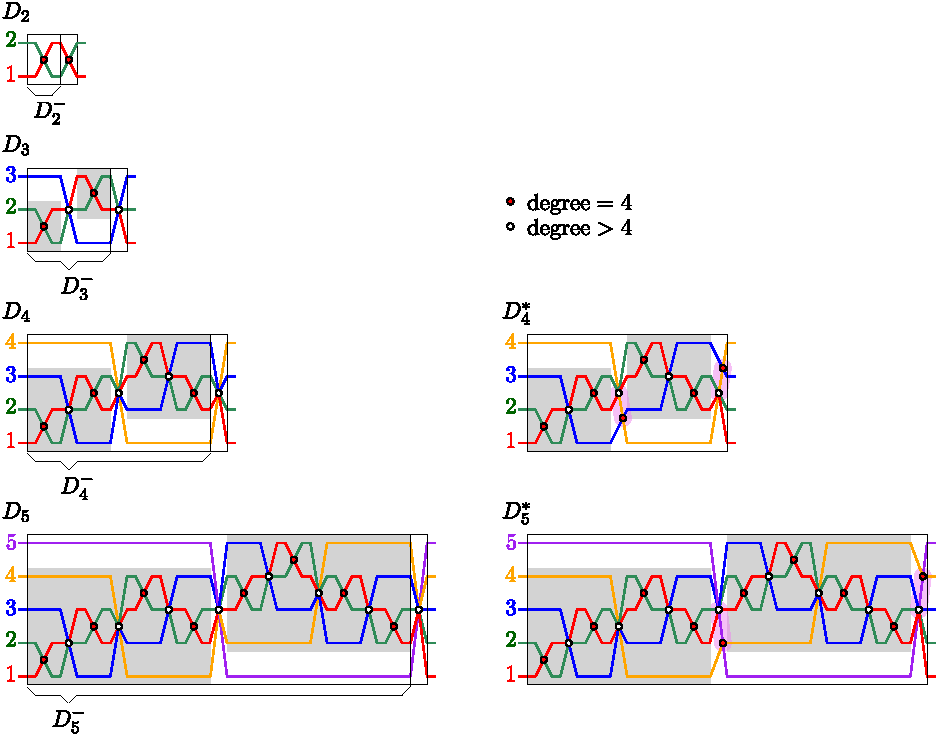
\includegraphics[width=0.7\linewidth,height=0.38\textheight,keepaspectratio]{graphics-page-7.pdf2svg.pdf}\end{center}
 Figure 10: Non-simple Venn diagrams $D_{n}$, $n\geq 2$, and $D_{n}^{*}$, $n\geq 4$, constructed in the proof of Theorem 6. Another drawing of $D_{4}^{*}$ is shown in Figure 6. 
% END S4.F10
% BEGIN S4.SS0.SSS0.P0.SPx1
\par\medskip\noindent\textbf{Proof of Theorem 6.}\par
% BEGIN S4.SS0.SSS0.P0.SPx1.p1
We inductively construct a family of non-simple monotone $n$-Venn diagrams $D_{n}$ for $n\geq 2$; see Figures 10 and 11. These are not the counterexamples yet, but those will be built from $D_{n}$ later by small modifications. Specifically, we describe $D_{n}$ as a wire diagram, i.e., each crossing occurs within a horizontally separated narrow vertical strip, and outside of these strips the $n$ curves are aligned to horizontal lines at heights $1,2,\ldots,n$. Furthermore, the diagram wraps around cylindrically at the left and right boundary. The curves are labeled $1,2,\ldots,n$ from bottom to top at the boundaries, according to their height.
\par
\par
% END S4.SS0.SSS0.P0.SPx1.p1
% BEGIN S4.F11
\begin{center}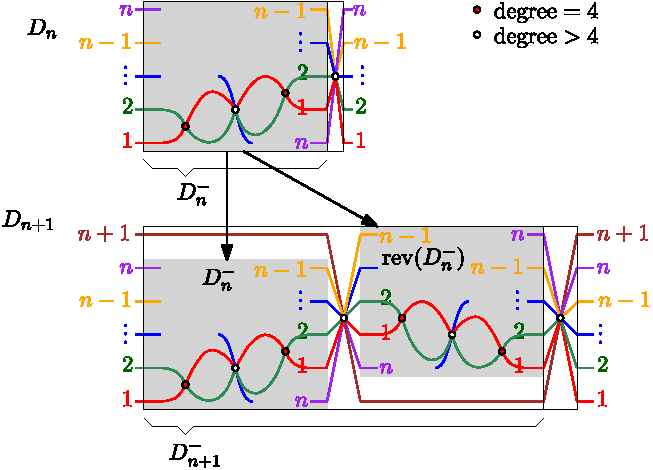
\includegraphics[width=0.7\linewidth,height=0.38\textheight,keepaspectratio]{graphics-page-8.pdf2svg.pdf}\end{center}
\par
 Figure 11: Illustration of the general inductive construction of $D_{n+1}$ from $D_{n}$. The reversed copy of $D_{n}^{-}$ is denoted $\operatorname{rev}(D_{n}^{-})$. 
% END S4.F11
% BEGIN S4.F12
\begin{center}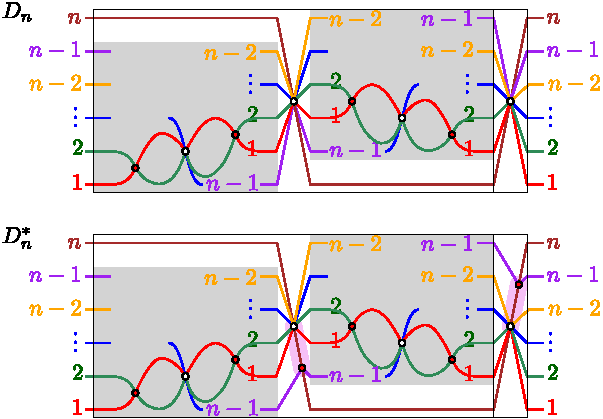
\includegraphics[width=0.7\linewidth,height=0.38\textheight,keepaspectratio]{graphics-page-9.pdf2svg.pdf}\end{center}
\par
 Figure 12: Modification of the diagram $D_{n}$ to obtain $D_{n}^{*}$ by slightly shifting the curve ${n-1}$. 
% END S4.F12
% BEGIN S4.SS0.SSS0.P0.SPx1.p2
For the induction basis $n=2$, we take $D_{2}$ as the wire diagram obtained from the unique Venn diagram with 2 curves, which has 2 crossings; see Figure 10. For the induction step $n\rightarrow n+1$, let $D_{n}^{-}$ be the diagram obtained from $D_{n}$ by removing the rightmost crossing. To construct $D_{n+1}$, we take a copy of $D_{n}^{-}$ vertically aligned at heights $1,\ldots,n$, a second copy of $D_{n}^{-}$ but reversed (mirrored along a vertical line, i.e., left and right are interchanged) to the right of the first copy and vertically aligned at heights $2,\ldots,n+1$; see Figure 11. We then add the curve $n+1$ starting on the left at height $n+1$ above the first copy of $D_{n}^{-}$, staying there until its right side, then crossing below the reversed second copy of $D_{n}^{-}$ to height 1, staying there until its right side, and finally crossing back up to height $n+1$ at the right boundary. The curves $1,\ldots,n$ are connected between the two copies of $D_{n}^{-}$ through one additional crossing with the curve $n+1$, and to the right of the second copy through a second additional crossing with the curve $n+1$, creating two additional crossings in total, so that the ordering of curves on the right boundary becomes $1,\ldots,n+1$, as desired. One can easily verify the following properties inductively:
\par
\begin{enumerate}
\item[]  (i) 
The total number of crossings in $D_{n}$ is $2^{n-1}$. In particular, the arrangement graph of $D_{n}$ has an even number of vertices.
\par
\par
\item[]  (ii) 
The subgraph of $D_{n}$ given by curve 1 and curve 2 contains all crossings, and exactly one pair of parallel edges between any two consecutive crossings. Every second crossing involves only the curves 1 and 2, i.e., the degree of the corresponding vertices is 4, and these vertices form an independent set.
\par
\par
\item[]  (iii) 
Exactly two of the crossings in $D_{n}$ involve all $n$ curves, i.e., the degree of the corresponding vertices is $2n$, and the clockwise cyclic orderings of the curves around the two crossings are $n-1,1,2,\ldots,n-2,n,n-2,\ldots,2,1,n-1,n$ and $n,1,2,\ldots,n-1,n,n-1,\ldots,2,1$, respectively.
\par
\par
\end{enumerate}
From (ii) we see in particular that the arrangement graph of $D_{n}$ has a perfect matching and a Hamilton cycle, i.e., it is not a counterexample to Conjecture 5. However, for $n\geq 4$ we can modify $D_{n}$ to obtain a diagram $D_{n}^{*}$ as follows; see Figure 12: From the first crossing involving all $n$ curves, we slightly shift down the curve $n-1$, and from the second crossing involving all $n$ curves, we slightly shift up the curve $n-1$, so that each of these two crossings is split into two, one of degree 4 and the other of degree $2n-2$ (this is possible because of (iii)). By (i), the number of vertices of $D_{n}^{*}$ is $2^{n-1}+2$, an even number. Furthermore, in the arrangement graph of $D_{n}^{*}$, let $U$ be the independent set of all degree 4 vertices and let $\overline{U}$ be its complement. From (ii) we obtain that $|U|=2^{n-1}/2+2=2^{n-2}+2$ and $|\overline{U}|=2^{n-1}/2=2^{n-2}$, and consequently $|U|>|\overline{U}|$. This inequality and the fact that $U$ is an independent set shows that $D_{n}^{*}$ does not have a perfect matching. This is the easy direction of Tutte’s theorem on perfect matchings. $\hfill\blacktriangleleft$
\par
\par
% END S4.SS0.SSS0.P0.SPx1.p2
% END S4.SS0.SSS0.P0.SPx1
% END S4
% BEGIN S5
\par\medskip\noindent\textbf{5 Open questions}\par
% BEGIN S5.p1
A natural question that remains open is whether Winkler’s conjecture holds for monotone Venn diagrams. We believe that the answer is “no”, but there are no counterexamples for $n\leq 6$ (recall Figure 4). One idea to find a monotone $n$-Venn quadrangulation without a perfect matching for $n\geq 7$ would be to extend the local obstruction $H$ highlighted in Figure 3, but so far we have not succeeded in this endeavor.
\par
\par
% END S5.p1
% BEGIN S5.p2
Computationally, it could be interesting to find all non-simple Venn diagrams for $n=4$ or $n=5$ curves and analyze their properties. What can be said about the asymptotic number of $n$-Venn diagrams as $n$ grows, or about the proportion of diagrams with certain properties?
\par
\par
% END S5.p2
% BEGIN S5.p3
In addition to these questions, there is a large number of other intriguing problems on Venn diagrams, concerning symmetry, convexity, number of crossings, restrictions on the allowed shapes of the curves (triangles, rectangles etc.), to be found in the survey [15]. For example, is there a simple $n$-Venn diagram with rotational symmetry made of $n$ congruent curves for every prime number $n$ (see [8, 11, 13])?
\par
\par
% END S5.p3
% END S5
% BEGIN bib
\par\medskip\noindent\textbf{References}\par
\begin{enumerate}
\item[]  [1]  Sofia Brenner, Linda Kleist, Torsten Mütze, Christian Rieck, and Francesco Verciani.  Disproving two conjectures on the Hamiltonicity of Venn diagrams, 2025.  URL: https://arxiv.org/abs/2503.18554.  
\item[]  [2]  Sofia Brenner, Torsten Mütze, and Francesco Verciani.  Venn Diagrams Program(s) and Output.  Software, swhId: swh:1:dir:baf5f66047caf6259cf73873956fbaf9305fa782 (visited on 2026-05-18).  URL: https://tmuetze.de/papers/venn.zip, doi:10.4230/artifacts.26092.  
\item[]  [3]  Bette Bultena, Branko Grünbaum, and Frank Ruskey.  Convex drawings of intersecting families of simple closed curves.  In Canadian Conference on Computational Geometry (CCCG), 1999.  URL: http://www.cccg.ca/proceedings/1999/c14.pdf.  
\item[]  [4]  Kiran B. Chilakamarri, Peter Hamburger, and Raymond E. Pippert.  Hamilton cycles in planar graphs and venn diagrams.  J. Comb. Theory B, 67(2):296–303, 1996.  doi:10.1006/JCTB.1996.0047.  
\item[]  [5]  Kiran B. Chilakamarri, Peter Hamburger, and Raymond E. Pippert.  Venn diagrams and planar graphs.  Geom. Dedicata, 62(1):73–91, 1996.  doi:10.1007/BF00240003.  
\item[]  [6]  Kiran B. Chilakamarri, Peter Hamburger, and Raymond E. Pippert.  Analysis of Venn diagrams using cycles in graphs.  Geom. Dedicata, 82(1-3):193–223, 2000.  doi:10.1023/A:1005288325189.  
\item[]  [7]  Stefan Felsner and Manfred Scheucher.  Arrangements of pseudocircles: Triangles and drawings.  Discret. Comput. Geom., 65(1):261–278, 2021.  doi:10.1007/S00454-020-00173-4.  
\item[]  [8]  Jerrold R. Griggs, Charles E. Killian, and Carla D. Savage.  Venn diagrams and symmetric chain decompositions in the boolean lattice.  Electron. J. Comb., 11(1), 2004.  doi:10.37236/1755.  
\item[]  [9]  Branko Grünbaum.  Venn diagrams. I.  Geombinatorics, 1(4):5–12, 1992.  
\item[]  [10]  Peter Hamburger and Raymond E. Pippert.  Simple, reducible Venn diagrams on five curves and Hamiltonian cycles.  Geom. Dedicata, 68(3):245–262, 1997.  doi:10.1023/A:1004924423245.  
\item[]  [11]  Charles E. Killian, Frank Ruskey, Carla D. Savage, and Mark Weston.  Half-simple symmetric Venn diagrams.  Electron. J. Comb., 11(1), 2004.  doi:10.37236/1839.  
\item[]  [12]  Khalegh Mamakani, Wendy Myrvold, and Frank Ruskey.  Generating simple convex Venn diagrams.  J. Discrete Algorithms, 16:270–286, 2012.  doi:10.1016/j.jda.2012.04.013.  
\item[]  [13]  Khalegh Mamakani and Frank Ruskey.  New roses: Simple symmetric Venn diagrams with 11 and 13 curves.  Discret. Comput. Geom., 52(1):71–87, 2014.  doi:10.1007/S00454-014-9605-6.  
\item[]  [14]  Gara Pruesse and Frank Ruskey.  All simple Venn diagrams are Hamiltonian, 2015.  doi:10.48550/arXiv.1504.06651.  
\item[]  [15]  Frank Ruskey and Mark Weston.  A survey of Venn diagrams.  Electron. J. Combin., 4(1):Dynamic Survey 5, 1997.  doi:10.37236/26.  
\item[]  [16]  Manfred Scheucher.  Pseudocircle arrangements tools, 2024.  GitHub repository: https://github.com/manfredscheucher/pseudocircle-arrangements-tools/.  
\item[]  [17]  William T. Tutte.  A theorem on planar graphs.  Trans. Amer. Math. Soc., 82:99–116, 1956.  doi:10.2307/1992980.  
\item[]  [18]  John Venn.  On the diagrammatic and mechanical representation of propositions and reasonings.  Phil. Mag. S. 5., 9(59):1–18, 1880.  doi:10.1080/14786448008626877.  
\item[]  [19]  Hassler Whitney.  A theorem on graphs.  Ann. of Math. (2), 32(2):378–390, 1931.  doi:10.2307/1968197.  
\item[]  [20]  Peter Winkler.  Venn diagrams: Some observations and an open problem.  Congr. Numer., 45:267–274, 1984.  
\item[]  [21]  Peter Winkler.  Mathematical puzzles: A connoisseur’s collection.  AK Peters Series, Taylor \& Francis, 2004.  
\item[]  [22]  Peter Winkler.  Puzzled: Where sets meet (Venn diagrams).  Commun. ACM, 55(2):128, 2012.  doi:10.1145/2076450.2076475.  
\end{enumerate}
% END bib

\end{document}
